\section{Checkpoint Selection Problem}\label{sec:partition}

\subsection{Problem Definition}

We consider a sequence of $n+1$ data $(d_0, \dots, d_n)$, where $d_0$ is the input and $d_n$ is the output, as in Section~\ref{sec:introduction}.
For ease of explanation, $d_i$ denotes both the data and the size of the data.
Since $d_0$ is the input and it needs to be in memory, we choose it as a checkpoint.
In addition, the training generates the output $d_n$ after the forward phase and immediately uses it at the beginning of the backward phase, so we cannot save any memory by {\em not} choosing it as a checkpoint.
As a result, without loss of generality, we assume both $d_0$ and $d_n$ are checkpoints in this paper.

\begin{figure}[h!tb]
\vspace*{5mm}
\begin{center}
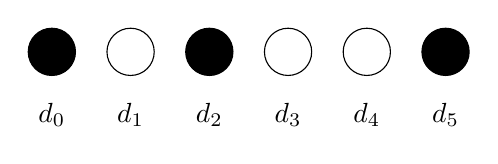
\begin{tikzpicture}
\draw[fill=black] (0,0) circle (0.3) node [black,yshift=-0.8cm] {$d_0$};
\draw[fill=none] (1,0) circle (0.3) node [black,yshift=-0.8cm] {$d_1$};
\draw[fill=black] (2,0) circle (0.3) node [black,yshift=-0.8cm] {$d_2$};
\draw[fill=none] (3,0) circle (0.3) node [black,yshift=-0.8cm] {$d_3$};
\draw[fill=none] (4,0) circle (0.3) node [black,yshift=-0.8cm] {$d_4$};
\draw[fill=black] (5,0) circle (0.3) node [black,yshift=-0.8cm] {$d_5$};
\end{tikzpicture}
\end{center}
\vspace*{-10mm}
\caption{An example of three checkpoints (in black) and two segments: \{d1\} and \{d3, d4\} (in white)} \label{fig:layers}
\end{figure}


Now we choose $m$ additional checkpoints to save memory by recomputing non-checkpoints during the backward phase, as in Algorithm~\ref{alg:train-checkpoint}.
Recall that the data between two checkpoints becomes a segment.
Now the set $C$ of $m + 2$ checkpoints (including $d_0$ and $d_n$)  will partition the sequence $(d_0, \dots, d_n)$ into $(s_1, \ldots, s_{m+1})$ segments, where each segment is the set of data between two checkpoints.
Note that two checkpoints may be adjacent so that a segment may be empty.
Figure~\ref{fig:layers} shows the partitioning of a model into three checkpoints and two segments.

From the previous discussion, we consider an objective function consisting of the {\em checkpoint memory} and the {\em segment memory}.
The {\em checkpoint memory} is the sum of the memory of all checkpoints, i.e., $\sum_{i \in C} d_i$.
The {\em segment memory} is the maximum of the sum of memory in every segment, i.e., $\max_i {\sum_{j \in s_i} d_j}$.
The goal is to find a checkpoint subset $C$ which minimizes the sum of checkpoint memory and segment memory (Equation~\ref{eq:cost}).
%The goal is to find a checkpoint subset $C$ that minimizes the sum of checkpoint memory and segment memory (Equation~\ref{eq:cost}).
We will denote this problem as the {\em checkpoint selection problem}.

\begin{equation}
\sum_{i \in C} d_i + \max_{1 \leq i \leq m+1}({\sum_{j \in s_i} d_j}) \label{eq:cost}
\end{equation}

\subsection{Dynamic Programming}

In this section, we solve the checkpoint selection problem by an algorithm based on dynamic programming.

The algorithm consists of two steps:
\begin{enumerate}
    \item For each possible segment memory $s$, find the minimal checkpoint memory $c_s$ such that the segment memory does not exceed $s$.
    \item Find the minimum of $s + c_s$.
\end{enumerate}
The implementation of step 2 is a simple algorithm iterating over all possible $s + c_s$.
In the next paragraph, we will discuss how to find $c_s$ for all $s$ in step 1.

Step 1 of the algorithm is implemented using dynamic programming as follows.
Define a function $M(i, s)$ as the minimum checkpoint memory for the sequence $(d_1, \ldots, d_i)$ such that the segment memory does not exceed $s$.
Here $c_s$ equals $M(n, s)$.
Now we derive the recursion for $M$.
%We first consider a more accessible version of the checkpoint selection problem in which we know the maximum segment memory.
%Let $s$ be the maximum segment memory allowed; how do we compute the minimum checkpoint memory?
%We derive dynamic programming that solves this problem for a segmented memory $s$.
%We define $M(i, s)$ as the minimum checkpoint memory for the sequence $(d_1, \ldots, d_i)$, subject to the condition that the segment memory is no more than $s$.
%Each $M(i, s)$ is the sum of the checkpoint $d_j$, closest to $d_i$, and the minimum checkpoint memory between $(d_1, \ldots, d_{j-1})$.
Each $M(i, s)$ is the sum of the checkpoint $d_j$, closest to $d_i$, and the minimum checkpoint memory between $(d_0, \ldots, d_{j-1})$.
%We now consider the possibility of choosing $d_j$ as a checkpoint.
Since the segment memory does not exceed $s$, the term $j$ must satisfy Inequality~\ref{ineq:j}.
%From the assumption that the segment memory is bounded by $s$, we have Inequality~\ref{ineq:j}.
%Note that we only consider $j$ so that the segment cost from $d_{j+1}$ to $d_{i}$ is no more than the segment cost $s$ we assumed.  
\begin{equation}
\sum_{k = j + 1}^i d_k \leq s \label{ineq:j}
\end{equation}
Therefore, the term $M(i, s)$ is the minimum of $d_j + M(j - 1, s)$ for all $j$ satisfying Equation~\ref{ineq:j}.
To express the recursion as a formula, let $l(i)$ be the minimum $j$ that satisfies Inequality~\ref{ineq:j}.
The recursion for $M$ is given in Equation~\ref{eq:T}.
%Now we consider all possible $j$'s that satisfy Inequality~\ref{ineq:j}.
%Let $l(i)$ be the minimum $j$ that satisfies Inequality~\ref{ineq:j}.
%Note that $l(i)$ is a non-decreasing function of $i$.
%We now derive the recursion for $M(i, s)$.

\begin{equation}
M(i, s) = \min_{l(i) \leq j \leq i} (d_j + M(j - 1, s)) \label{eq:T}
\end{equation}

\begin{algorithm}[h!tb]
\begin{algorithmic}
\caption{Checkpoint Selection}
\label{alg:checkpoint-selection}
%\Comment{Forward phase}
\Require data sizes $d_0, \ldots, d_n$.
\Ensure The minimum cost of checkpoint selection
\For{all segment cost $s$}
    \State{Compute each $l(i)$ for $1 \leq i \leq n$}
    \State{$M(0, s) = d_0$}
%   \State{$M(s, 0) = d_0$}
    \State{$Q = \{0\}$}
    \For{$i \gets 1$ to $n$}
%        \State {Remove those $q_h$ from the head of $Q$ such that $l(i) > j$.}
        \State {Remove those $q_h$ from the head of $Q$ such that $l(i) > q_h$.}
        \State {Set $M(i, s)$ to be $d_q + M(q - 1, s)$, where $q$ is the head of $Q$.}
        \State {Remove those $q_t$ from the tail of $Q$ such that $d_{q_t} + M(q_t - 1, s) > d_i + M(i - 1, s)$.}
        \State {Add $i$ to the tail of $Q$.}
    \EndFor
%    \State{$Q = \emptyset$}
%    \For{$i \gets 1$ to $n$}
%        \State {Remove from the end of $Q$ those element greater than $d_i + M(i - 1, s)$}
%        \State {Add $d_i + M(i - 1, s)$ to the tail of $Q$}
%        \State {Set $M(i, s)$ to be the first element of $Q$}
%    \EndFor        
\EndFor
\State{return $\min_{s} (s + M(n, s))$} \Comment{the answer}
\end{algorithmic}
\end{algorithm}

Algorithm~\ref{alg:checkpoint-selection} is the implementation details of the algorithm that solves the checkpoint selection problem.
%We can now use Equation~\ref{eq:T} to solve the checkpoint selection problem as in Algorithm~\ref{alg:checkpoint-selection}.
%First, we enumerate all possible segment cost $s$, then we use Equation~\ref{eq:T} to solve $M(n, s)$ for this given $s$.
%Finally, we find the minimum among all $M(n, s)$ for all $s$, which is the answer to our checkpoint selection problem.
%We will analyze the time complexity of using Equation~\ref{eq:T} to solve $M(n, s)$ for a given $s$, and the number of segment costs $s$ we need to enumerate in the following two paragraphs.
%The head of $Q$, say $q$, must be the one with the smallest $d_q + M(q - 1, s)$ since each time we add an element $u$ to $Q$, we remove those $v$ from the end of $Q$ such that $d_u + M(u - 1, s) < d_v + M(v - 1, s)$.
%Therefore, we have $M(i, s) = d_q + M(q - 1, s)$.
% We use a queue $Q$, which contains the $j$'s in Equation~\ref{eq:T}, to implement the recursion of $M$.
We claim that, in order to prove the correctness of our algorithm,
\begin{itemize}
    \item the queue $Q$ contains the $j$'s achieving the minimum in Equation~\ref{eq:T}, and
%    \item the head of $Q$ is such a $j$.
    \item the head of $Q$ is $\displaystyle\argmin_{l(i)\leq j\leq i}\,(d_j + M(j - 1, s))$.
\end{itemize}

The latter is valid, since in the $i$-th iteration, we remove those $j$ from the tail of $Q$ such that $d_i + M(i - 1, s) < d_j + M(j - 1, s)$.
Therefore, the head of $Q$, say $q$, is the element with the smallest $d_q + M(q - 1, s)$ in $Q$.

To prove the former, we ensure that in the $i$-th iteration, all $j$'s with $j < i$ have entered $Q$, and only the ones that do not achieve the minimum in Equation~\ref{eq:T} are removed from $Q$.
All $j$'s with $j < i$ have entered $Q$ since we add each $j$ to the tail of $Q$ before the end of the $j$-th iteration.
If $u < i$ is removed from $Q$ because some $v < i$ induces $u < l(v)$, then since $l$ is monotonically increasing, we have $l(v) < l(i)$, implying that $u < l(i)$.
Therefore, the term $u$ is not a valid $j$ in Equation~\ref{eq:T}.
If $u < i$ is removed from $Q$ because some $v < i$ induces $d_u + d(u - 1, s) > d_v + d(v - 1, s)$, then whenever $u$ is a valid $j$ in Equation~\ref{eq:T}, we can always find another $j$, namely $v$, with a smaller $d_j + M(j - 1, s)$.
Therefore, the term $u$ is not the $j$ achieving the minimum in Equation~\ref{eq:T}.

We analyze the time complexity of Algorithm~\ref{alg:checkpoint-selection} in the following paragraphs.
To analyze the time complexity of completing the recursion $M(i, s)$ for a fixed $s$, three operations are put into consideration: computing each $l(i)$ with $1 \leq i\leq n$, assigning values to each $M(i, s)$, and maintaining the queue $Q$.
%To analyze the time complexity of completing the recursion $M(i, s)$ for a fixed $s$, two operations are put into consideration: assigning values to each $M(i, s)$ and maintaining the queue $Q$.
\begin{itemize}
\item Computing each $l(i)$ takes $O(n)$ time by maintaining the sliding window that starts at $l(i)$ and ends at $i$ over the sequence $(1, 2,\dots, n)$.
This is because each element in the sequence $(0, 1,\dots, n)$ enters and exits the window only once, and each insertion and deletion takes $O(1)$ time.
\item In the $i$-th iteration for each segment memory usage $s$, it takes $O(1)$ time to find the head of $Q$, say $q$, and assign $d_q + M(q - 1, s)$ to each $M(i, s)$.
Therefore, it takes $O(n)$ time to assign values to each $M(i, s)$ for a fixed $s$.
%\item For each segment memory usage $s$, each number from $0$ to $n$ enters and leaves the queue $Q$ once, and therefore it takes $O(n)$ time to maintain the queue $Q$.
\item For each segment memory usage $s$, each number from $0$ to $n$ enters and leaves the queue $Q$ once, resulting in $O(n)$ insertions and deletions.
Since each insertion and deletion occurs only at the head and tail of $Q$, both operations have $O(1)$ time complexity.
Therefore, the maintenance of $Q$ takes $O(n)$ time.
\end{itemize}
As a result, it takes $O(n)$ time to complete the recursion of $M(i, s)$ for a fixed $s$.

Next, we find the number of different segment memory usages.
%The next question is determining the segment cost $s$ for $M$ in Equation~\ref{ineq:j} and \ref{eq:T}.
We cannot iterate each value between $1$ and $\sum_{i = 1}^n d_i$ since it leads to a pseudo-polynomial time algorithm.
%We cannot test all possible values below $\sum_{i = 1}^n d_i$ since it leads to a pseudo-polynomial time algorithm, not a polynomial-time algorithm.
In fact, there are $O(n^2)$ possible segment memory usages, obtained by enumerating the start and end points of the segments.
%Instead, we observe only $O(n^2)$ possible segments since every segment has a starting and end point.

As a result, there are $O(n^2)$ different segment memory usages, each taking $O(n)$ time to compute.
%Therefore, Theorem~\ref{thm:checkpoint-selection-problem} follows.
Therefore, we obtain the following theorem.
%As a result, we only need to consider $O(n^2)$ different $s$'s in Equation~\ref{ineq:j} and \ref{eq:T}.
%We also know that the time complexity for computing $T$ with a given $s$ is $O(n)$ from the previous discussion; therefore, we conclude that the total time for solving the checkpoint selection problem is $O(n^3)$.

%After knowing all $M$ function values, we can solve the checkpoint selection problem by finding the $s$ that minimizes Equation~\ref{eq:sol}, where $s$ is the segment memory and $M(n, s)$ is the checkpoint memory.

%\begin{equation}
%\min_{s} (s + M(n, s) \label{eq:sol})
%\end{equation}

\begin{theorem}
\label{thm:checkpoint-selection-problem}
The checkpoint selection problem is $O(n^3)$-time solvable, where $n$ is the number of neural network layers.
%A dynamic program solves the checkpoint selection problem in $O(n^3)$ time, where $n$ is the number the neural network layers.
\end{theorem}